% This is an appendix, it behaves like an ordinary chapter
% appendices are nice places to put things like proofs that are
% too ugly to keep in the body of the thesis and things like
% code or data that no one really wants to look at


%-----------------------------------------------------
\chapter{Appendix}
\VerbatimInput{TestFile.txt}
%-----------------------------------------------------
% 4     3     2     1\newline     
% $\vert$-----$\vert$     |-----|\newline

%%\dividepage
%%\chapter{Extra Material}
%%\VerbatimInput{MinLaddersPrint.txt}
\input{MinLaddersPrint.txt}
\pagebreak
\input{textTable.txt}

\subsection{Axillary Functions and Details for {\sc FindAllChildren}}
\subsubsection{Local Swap Operation}

The parent-child relation in the tree structure for {\sc FindAllChildren} is based on a \emph{local swap operation} 
which corresponds to a braid relation and is a local modification of $ladder$ as shown in Figure~\ref{fig:rightSwap}.
To get from the parent to the child a right swap operation is performed. To get from the child to the parent 
a left swap operation is performed. 
Given an arbitrary bar, $x$, it can be right swapped if and only if there are two bars, $y,z$ where $y \neq z$ 
such that all the following conditions are met~\cite{A1}.
\begin{itemize}
	\item The left end point of $z$ is directly above the left end point of $x$.
	\item The left end point of $y$ is directly above the right end point if $x$.
	\item The right end point of $z$ is directly above the left end point of $y$.
\end{itemize}

Given an arbitrary bar, $x$, it can be left swapped if and only if there are two bars, $y,z$ where $y \neq z$ 
such that the following conditions are met~\cite{A1}.
\begin{itemize}
	\item The right end point of $z$ is directly below the right end point of $x$.
	\item The right end point of $y$ is directly below the left end point if $x$.
	\item The left end point of $z$ is directly below the right end point of $y$.
\end{itemize}
In the left ladder in Figure~\ref{fig:rightSwap} bar $x=(3,1)$, bar $y=(5,1)$ and bar $z=(5,3)$. Bar $x$ can be right swapped 
seeing as the three conditions for performing a right swap operation are met.
In the right ladder in Figure~\ref{fig:rightSwap} bar $x=(3,1)$, bar $y=(5,1)$ and bar $z=(5,3)$. Bar $x$ can be left swapped 
seeing as the three conditions for performing a left swap operation are met.
\begin{figure}[h]
	\begin{minipage}{0.4\textwidth}
		\begin{center}

			%%drawing the lines
			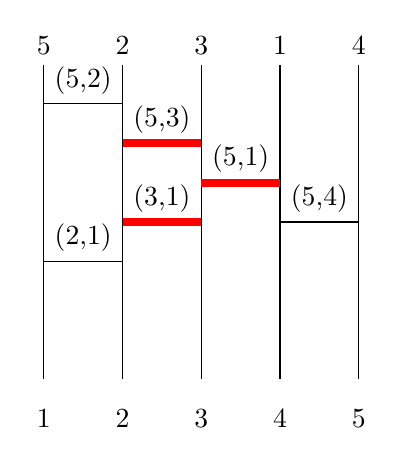
\begin{tikzpicture}
				\draw(0, 0) to (0, 4) node[above]{5};
				\node at (0, -0.5){1};

				\draw(1, 0) to (1, 4) node[above]{2};
				\node at (1, -0.5){2};


				\draw(2, 0) to (2, 4) node[above]{3};
				\node at (2, -0.5){3};

				\draw(3, 0) to (3, 4) node[above]{1};
				\node at (3, -0.5){4};


				\draw(4, 0) to (4, 4) node[above]{4};
				\node at (4, -0.5){5};

				%%drawing the bars

				%%5's route
				\draw(0, 3.5)to (1, 3.5);
					\draw node at (0.5, 3.8) {(5,2)};
				\draw[line width=1mm, red](1, 3) to (2, 3);
					\draw node at (1.5, 3.3) {(5,3)};
				\draw[line width=1mm, red](2, 2.5) to (3, 2.5);
					\draw node at (2.5, 2.8) {(5,1)};
				\draw(3, 2) to (4, 2);
					\draw node at (3.5, 2.3) {(5,4)};

				%%4's route, no bars

				%%3s route
				\draw[line width=1mm, red](1, 2) to (2, 2);
					\draw node at (1.5, 2.3) {(3,1)};
				%%2s route
				\draw(0, 1.5) to (1, 1.5);
					\draw node at (0.5, 1.8){(2,1)};

			\end{tikzpicture}
		\end{center}
	\end{minipage}
	\begin{minipage}{0.4\textwidth}
		\begin{flushright}

			%%drawing the lines
			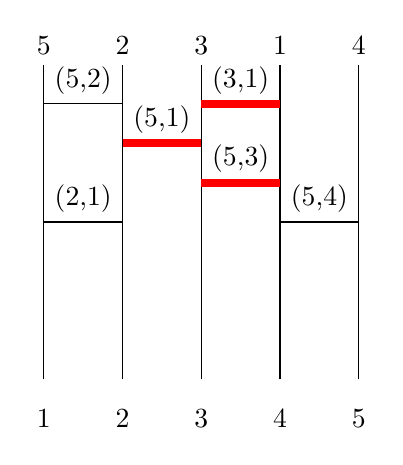
\begin{tikzpicture}
				\draw(0, 0) to (0, 4) node[above]{5};
				\node at (0, -0.5){1};

				\draw(1, 0) to (1, 4) node[above]{2};
				\node at (1, -0.5){2};


				\draw(2, 0) to (2, 4) node[above]{3};
				\node at (2, -0.5){3};

				\draw(3, 0) to (3, 4) node[above]{1};
				\node at (3, -0.5){4};


				\draw(4, 0) to (4, 4) node[above]{4};
				\node at (4, -0.5){5};

				%%Drawing the bars
				\draw(0, 3.5)to (1, 3.5);
					\draw node at (0.5, 3.8){(5,2)};
				\draw[line width=1mm, red](2, 3.5) to (3, 3.5);
					\draw node at (2.5, 3.8) {(3,1)};
				\draw[line width=1mm, red](2, 2.5) to (3, 2.5);
					\draw node at (2.5, 2.8) {(5,3)};
				\draw(3, 2) to (4, 2);
					\draw node at (3.5, 2.3){(5,4)};
				%%4's route, no bars

				%%3s route
				\draw[line width=1mm, red](1, 3) to (2, 3);
					\draw node at (1.5, 3.3) {(5,1)};
				%%2s route
				\draw(0, 2) to (1, 2);
					\draw node at(0.5, 2.3){(2,1)};
			\end{tikzpicture}
		\end{flushright}
	\end{minipage}
	\caption{Example of a local swap operation. When a right swap operation is performed
	on the left ladder, the result is the right ladder. When a left swap operation is performed
	on the right ladder, the result is the left ladder.}
	\label{fig:rightSwap}
\end{figure}


The following algorithms are used to perform a local swap operation: Algorithm~\ref{Alg:RightSwap}, Algorithm~\ref{Alg:LeftSwap} and Algorithm~\ref{Alg:ShiftSubLadder}.
Let $ladder$ be initialized to an empty ladder. Let $bar$ be the bar to be right or left swapped in the $ladder$.
In Algorithm~\ref{Alg:ShiftSubLadder} \textit{offset} is initialized to $2$ when right swapping and initialized to 
$-2$ when left swapping. In Algorithm~\ref{Alg:ShiftSubLadder} \textit{index} is initialized to $1$ when 
right swapping and $-1$ when left swapping.
Let the \emph{right child} of some arbitrary bar $w$, $rc(w)$ for short, be the bar one row below, and one column to the 
right of $w$. Let the \emph{left child} of some arbitrary bar $w$, $lc(w)$ for short, be the bar one 
row below, and one column to the left of $w$. 
Let the \emph{right sibling} of $w$, $rs(w)$ for short,  be defined as the bar on the same row as some arbitrary bar $w$ and
two columns to the right of bar $w$. 
Let the \emph{upper neighbor} of $w$, $un(w)$ for short, be the bar that is two rows above the row of $w$ and is 
in the same column as $w$. Let the \emph{right neighbor} of $w$, $rn(w)$ for short, be the bar that is one row 
above $w$ and one column to the right of $w$. Let the lower neighbor of $w$, $ln(w)$ for short be 
the bar that is two rows below $w$ and in the same column as $w$. Let the left neighbor of 
$w$, $lfn(n)$ for short, be the bar one row below and one column to the left of $w$.
Let the \emph{sub-ladder} be a subset of bars such that each bar in the sub-ladder is a left or right child 
of some other bar in the sub-ladder except the root of the sub-ladder. For an example of a sub-ladder please refer to 
Figure~\ref{Figure:Sub-ladder}.
\begin{figure}[h]
	\centering
	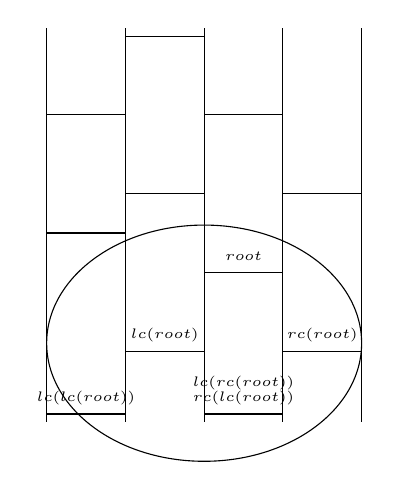
\begin{tikzpicture}
		\draw(0, 0) to (0, 5);
			\draw(0, 3.9) to (1, 3.9);
			\draw(0, 2.4) to (1, 2.4);
			\node at(.5, .3){\tiny{$lc(lc(root))$}};
			\draw(0, 0.1) to (1, 0.1);
		\draw(1, 0) to (1, 5);
			\draw(1, 4.9) to (2, 4.9);
			\draw(1, 2.9) to (2, 2.9);
			\node at(1.5, 1.1){\tiny{$lc(root)$}};
			\draw(1, 0.9) to (2, 0.9);
		\draw(2, 0) to (2, 5);
			\draw(2, 3.9) to (3, 3.9);
			\node at(2.5, 2.1){\tiny{$root$}};
			\draw(2, 1.9) to (3, 1.9);
			\node at(2.5, .3){\tiny{$rc(lc(root))$}};
			\node at(2.5, .5){\tiny{$lc(rc(root))$}};
			\draw(2, 0.1) to (3, 0.1);
		\draw(3, 0) to (3, 5);
			\draw(3, 2.9) to (4, 2.9);
			\node at(3.5,1.1){\tiny{$rc(root)$}};
			\draw(3, 0.9) to (4, 0.9);
		\draw(4, 0) to (4, 5);

		\draw (2, 1) ellipse (2cm and 1.5cm);
	\end{tikzpicture}

	\caption{The bars that are fully or partially in the circle make up the sub-ladder.}
	\label{Figure:Sub-ladder}
	
\end{figure}

%%%%%%% ALGORITHM RIGHT SWAP %%%%%%%%%%%%%%%%%%%
\begin{algorithm}[!htp]
	\begin{algorithmic}[1]
		\Function{RightSwap}{$ladder$, $bar$}
			\State $row \gets bar's$ row in $ladder$
			\State $col \gets bar's$ column in $ladder$
			\State $upperNeighbor \gets un(bar)$
			\State $rightNeighbor \gets rn(bar)$
			\If{$col<=n-3$}
				\State $subLadderRoot \gets$ $rs(bar)$
				\State {\sc ShiftSubLadder($ladder$, $subLadderRoot$, 2)}
			\EndIf
			\State {\sc Swap($upperNeighbor$, $ladder[row+1][col+1]$)}
			\State {\sc Swap($bar$, $rightNeighbor$)}
		\EndFunction
	\end{algorithmic}
	\caption{Perform a right swap operation on a bar}
	\label{Alg:RightSwap}
\end{algorithm}


%%%%%%%%%% ALGORITHM LEFT SWAP %%%%%%%%%%%%%%%%%%%%%%%%
\begin{algorithm}[!htp]
	\begin{algorithmic}[1]
		\Function{LeftSwap}{$ladder$, $bar$}
			\State $row \gets bar's$ row in ladder 
			\State $col \gets bar's$ column in ladder
			\State $leftNeighbor \gets lfn(bar)$
			\State {\sc Swap($bar$, $leftNeighbor$)}
			\State $lowerNeighbor \gets ln(bar)$
			\If{$col<n-1$}
				\State $subLadderRoot \gets$ $rc(lowerNeighbor)$
				\State {\sc Swap($lowerNeighbor$, $ladder[row-1][col-1]$)}
				\State {\sc ShiftSubLadder($ladder$, $subLadderRoot$, $-2$)}
			\Else 
				\State {\sc Swap($lowerNeighbor$, $ladder[row-1][col-1]$)}
			\EndIf
		\EndFunction
	\end{algorithmic}
	\caption{Perform a left swap operation on a bar}
	\label{Alg:LeftSwap}
\end{algorithm}


%%%%%%%%%%%% ALGORITHM ShiftSubLadderDOWN %%%%%%%%%%%%%%%%%%%%%%
\begin{algorithm}[!htp]
	\begin{algorithmic}[1]
		\Function{ShiftSubLadder}{$ladder$, $bar$, \textit{offset}}
			\State $row \gets bar's$ row in ladder
			\State $col \gets bar's$ column in ladder
			\State $rightChild \gets rc(bar)$
			\State $leftChild \gets lc(bar)$
			\If{$rightChild=0$ \textbf{and} $leftChild=0$}
				\State {\sc Swap($ladder[row+$\textit{offset}$][col]$, $ladder[row][col]$)}
				\State \textbf{return}
			\Else 
				\If{\textit{offset}$==-2$ indicating a left swap}
					\State {\sc Swap($ladder[row+$\textit{offset}$][col]$, $ladder[row][col]$)}
					\If{$rightChild \neq 0$}
						\State {\sc ShiftSubLadder($ladder$, $rightChild$, \textit{offset})}
					\EndIf 
					\If{$leftChild \neq 0$}
						\State {\sc ShiftSubLadder($ladder$, $leftChild$, \textit{offset})}
					\EndIf
				\EndIf
				\If{\textit{offset}$==2$ indicating a right swap}
					\If{$rightChild \neq 0$}
						\State {\sc ShiftSubLadder($ladder$, $rightChild$, \textit{offset})}
					\EndIf 
					\If{$leftChild \neq 0$}
						\State {\sc ShiftSubLadder($ladder$, $leftChild$, \textit{offset})}
					\EndIf 
					\State {\sc Swap($ladder[row+$\textit{offset}$][col]$, $ladder[row][col]$)}
				\EndIf
			\EndIf
		\EndFunction
	\end{algorithmic}
	\caption{Shifts the sub-ladder up or down the ladder data structure depending on if a right or left swap operation is being performed}
	\label{Alg:ShiftSubLadder}
\end{algorithm}\pagebreak


The way that the aforementioned three algorithms work in order 
to complete a local swap operation is as follows. 
When performing a right swap operation, {\sc RightSwap}
takes the current bar, $x$, and gets its upper neighbor $z$ and its right neighbor $y$; $x$, $z$ and $y$ meet the 
criteria for performing a right swap operation. Then, {\sc RightSwap} calls {\sc ShiftSubLadder}
with the \emph{offset} value of $2$ and the \emph{index} value of one. 
Algorithm {\sc ShiftSubLadder} ensures that the bottom right sub-ladder, beginning at the right sibling of $x$/$rs(x)$, 
is shifted down the ladder such that when the right 
swap operation is performed, the root of the sub-ladder is the right child of $z$. 
When performing a right swap, {\sc ShiftSubLadder} moves each bar in the sub-ladder two rows 
down the ladder. Since each bar in the sub-ladder is a left or right child of some other bar in the sub-ladder, 
with the exception of the root ladder, the index is set to $1$ indicating the offset.
When a right swap operation is about to occur, bar $z$ will be moved from its current row and column to its current row + $3$ 
and its current column $+1$. Once the right swap operation is performed, 
$rs(x)$ becomes $rc(z)$. $y$ and $x$ are swapped. Then the function is complete.\par 

The left swap operation reverses the resulting ladder from the right swap operation; {\sc LeftSwap}
is the inverse of {\sc RightSwap}. The \textit{offset} value for {\sc ShiftSubLadder} when 
performing a left swap is set to $-2$ to indicate the bars need to be moved up the ladder. 
When bars are moved in {\sc LeftSwap}, the parent bar is shifted upward before its children.
This is unlike the {\sc RightSwap} in which the children bars are shifted downward 
before their parent. This is done to ensure that for any two bars in the sub-ladder, 
$x,y$, $x$ will not be swapped with $y$, thus putting $y$ in the wrong position. 
This is why the $lowerNeighbor$ of $x$ in {\sc LeftSwap} is swapped before 
{\sc ShiftSubLadder} is called. Whereas in {\sc RightSwap} the $upperNeighbor$ 
of $x$ is swapped after {\sc ShiftSubLadder} is called.
To see an example of all three algorithms performing a local swap operation please refer to Figure \ref{Fig:SwapAndShift}.\pagebreak
\begin{figure}[!htp]
	\begin{minipage}{.4\textwidth}
		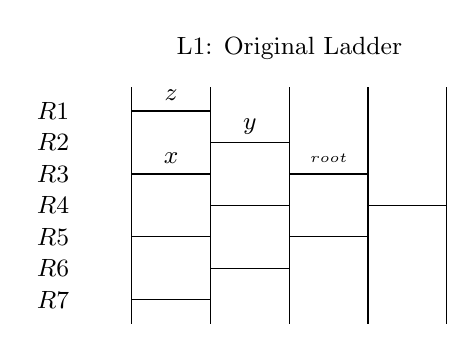
\begin{tikzpicture}
			\node at(2, 3.5){\small{L1: Original Ladder}};
			\draw(0, 0) to (0, 3);
					\node at(.5, 2.9){\small{$z$}};
				\draw(0, 2.7) to (1,2.7);
					\node at(.5, 2.1){\small{$x$}};

				\draw(0,1.9) to (1,1.9);
				\draw(0,1.1) to (1,1.1);
				\draw(0,0.3) to (1,0.3);
			\draw(1, 0) to (1, 3);
				\node at(1.5,2.5){\small{$y$}};
				\draw(1,2.3) to (2,2.3);
				\draw(1,1.5) to (2,1.5);
				\draw(1,0.7) to (2,0.7);
			\draw(2, 0) to (2, 3);
				\node at(2.5, 2.1){\tiny{$root$}};
				\draw(2,1.9) to (3,1.9);
				\draw(2,1.1) to (3,1.1);
			\draw(3, 0) to (3, 3);
				\draw(3,1.5) to (4,1.5);
			\draw(4, 0) to (4, 3);

			\node at(-1, 2.7){\small{$R1$}};
			\node at(-1, 2.3){\small{$R2$}};
			\node at(-1, 1.9){\small{$R3$}};
			\node at(-1, 1.5){\small{$R4$}};
			\node at(-1, 1.1){\small{$R5$}};
			\node at(-1, .7){\small{$R6$}};
			\node at(-1, .3){\small{$R7$}};

			
		\end{tikzpicture}
	\end{minipage}
	\begin{minipage}{.4\textwidth}
		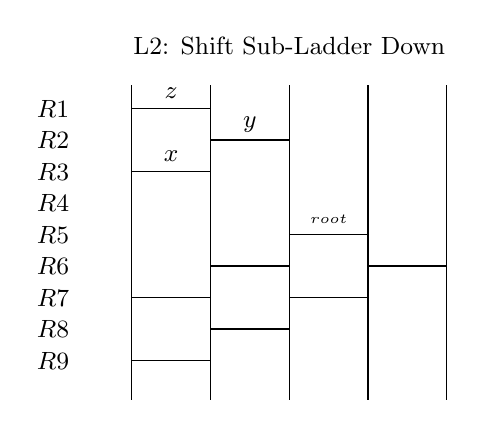
\begin{tikzpicture}
			\node at(2, 3.5){\small{L2: Shift Sub-Ladder Down}};

			\draw(0, -1) to (0, 3);
					\node at(.5, 2.9){\small{$z$}};
				\draw(0, 2.7) to (1,2.7);
					\node at(.5, 2.1){\small{$x$}};

				\draw(0,1.9) to (1,1.9);
				\draw(0,.3) to (1,.3);
				\draw(0,-0.5) to (1,-0.5);
			\draw(1, -1) to (1, 3);
				\node at(1.5,2.5){\small{$y$}};
				\draw(1,2.3) to (2,2.3);
				\draw(1,0.7) to (2,0.7);
				\draw(1,-0.1) to (2,-0.1);
			\draw(2, -1) to (2, 3);
				\node at(2.5, 1.3){\tiny{$root$}};
				\draw(2,1.1) to (3,1.1);
				\draw(2,.3) to (3,.3);
			\draw(3, -1) to (3, 3);
				\draw(3,.7) to (4,.7);
			\draw(4, -1) to (4, 3);

			\node at(-1, 2.7){\small{$R1$}};
			\node at(-1, 2.3){\small{$R2$}};
			\node at(-1, 1.9){\small{$R3$}};
			\node at(-1, 1.5){\small{$R4$}};
			\node at(-1, 1.1){\small{$R5$}};
			\node at(-1, .7){\small{$R6$}};
			\node at(-1, .3){\small{$R7$}};
			\node at(-1, -.1){\small{$R8$}};
			\node at(-1, -.5){\small{$R9$}};


			
		\end{tikzpicture}
	\end{minipage}
	\begin{minipage}{.4\textwidth}
		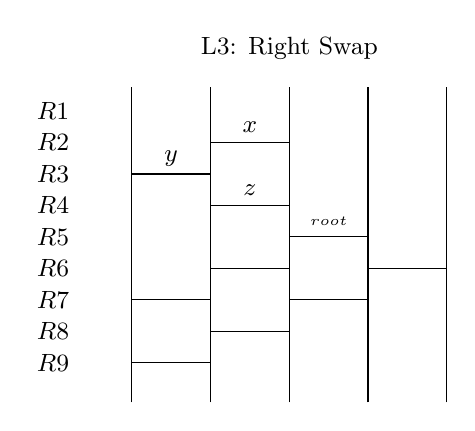
\begin{tikzpicture}
			\node at(2, 3.5){\small{L3: Right Swap}};

			\draw(0, -1) to (0, 3);
					\node at(1.5, 1.7){\small{$z$}};
				
					\node at(.5, 2.1){\small{$y$}};

				\draw(0,1.9) to (1,1.9);
				\draw(0,.3) to (1,.3);
				\draw(0,-0.5) to (1,-0.5);
			\draw(1, -1) to (1, 3);
				\node at(1.5,2.5){\small{$x$}};
				\draw(1,2.3) to (2,2.3);
				\draw(1, 1.5) to (2,1.5);
				\draw(1,0.7) to (2,0.7);
				\draw(1,-0.1) to (2,-0.1);
			\draw(2, -1) to (2, 3);
				\node at(2.5, 1.3){\tiny{$root$}};
				\draw(2,1.1) to (3,1.1);
				\draw(2,.3) to (3,.3);
			\draw(3, -1) to (3, 3);
				\draw(3,.7) to (4,.7);
			\draw(4, -1) to (4, 3);

			\node at(-1, 2.7){\small{$R1$}};
			\node at(-1, 2.3){\small{$R2$}};
			\node at(-1, 1.9){\small{$R3$}};
			\node at(-1, 1.5){\small{$R4$}};
			\node at(-1, 1.1){\small{$R5$}};
			\node at(-1, .7){\small{$R6$}};
			\node at(-1, .3){\small{$R7$}};
			\node at(-1, -.1){\small{$R8$}};
			\node at(-1, -.5){\small{$R9$}};


			
		\end{tikzpicture}
	\end{minipage}
	\hfill
	\begin{minipage}{.4\textwidth}
		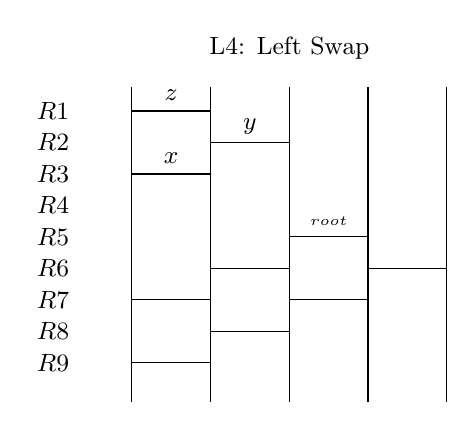
\begin{tikzpicture}
			\node at(2, 3.5){\small{L4: Left Swap}};

			\draw(0, -1) to (0, 3);
					\node at(0.5, 2.9){\small{$z$}};
				
					\node at(.5, 2.1){\small{$x$}};

				\draw(0,1.9) to (1,1.9);
				\draw(0,.3) to (1,.3);
				\draw(0,-0.5) to (1,-0.5);
			\draw(1, -1) to (1, 3);
				\node at(1.5,2.5){\small{$y$}};
				\draw(1,2.3) to (2,2.3);
				\draw(0, 2.7) to (1,2.7);
				\draw(1,0.7) to (2,0.7);
				\draw(1,-0.1) to (2,-0.1);
			\draw(2, -1) to (2, 3);
				\node at(2.5, 1.3){\tiny{$root$}};
				\draw(2,1.1) to (3,1.1);
				\draw(2,.3) to (3,.3);
			\draw(3, -1) to (3, 3);
				\draw(3,.7) to (4,.7);
			\draw(4, -1) to (4, 3);

			\node at(-1, 2.7){\small{$R1$}};
			\node at(-1, 2.3){\small{$R2$}};
			\node at(-1, 1.9){\small{$R3$}};
			\node at(-1, 1.5){\small{$R4$}};
			\node at(-1, 1.1){\small{$R5$}};
			\node at(-1, .7){\small{$R6$}};
			\node at(-1, .3){\small{$R7$}};
			\node at(-1, -.1){\small{$R8$}};
			\node at(-1, -.5){\small{$R9$}};
		\end{tikzpicture}
	\end{minipage}
	\begin{center}
	 \begin{minipage}{.5\textwidth}
	 	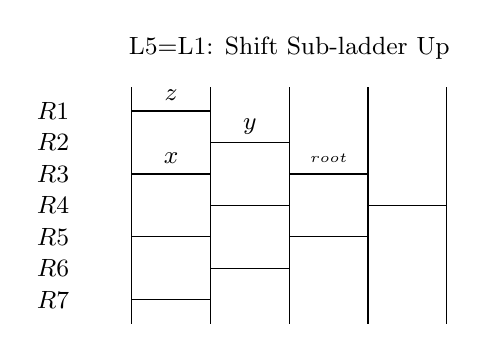
\begin{tikzpicture}
	 		\node at(2, 3.5){\small{L5=L1: Shift Sub-ladder Up}};
	 		\draw(0, 0) to (0, 3);
	 				\node at(.5, 2.9){\small{$z$}};
	 			\draw(0, 2.7) to (1,2.7);
	 				\node at(.5, 2.1){\small{$x$}};

	 			\draw(0,1.9) to (1,1.9);
	 			\draw(0,1.1) to (1,1.1);
	 			\draw(0,0.3) to (1,0.3);
	 		\draw(1, 0) to (1, 3);
	 			\node at(1.5,2.5){\small{$y$}};
	 			\draw(1,2.3) to (2,2.3);
	 			\draw(1,1.5) to (2,1.5);
	 			\draw(1,0.7) to (2,0.7);
	 		\draw(2, 0) to (2, 3);
	 			\node at(2.5, 2.1){\tiny{$root$}};
	 			\draw(2,1.9) to (3,1.9);
	 			\draw(2,1.1) to (3,1.1);
	 		\draw(3, 0) to (3, 3);
	 			\draw(3,1.5) to (4,1.5);
	 		\draw(4, 0) to (4, 3);

	 		\node at(-1, 2.7){\small{$R1$}};
	 		\node at(-1, 2.3){\small{$R2$}};
	 		\node at(-1, 1.9){\small{$R3$}};
	 		\node at(-1, 1.5){\small{$R4$}};
	 		\node at(-1, 1.1){\small{$R5$}};
	 		\node at(-1, .7){\small{$R6$}};
	 		\node at(-1, .3){\small{$R7$}};

		
	 	\end{tikzpicture}
	 \end{minipage}
	 \end{center}
	\caption{$x,y,z$ to be locally swapped. $root$ is the root of the sub-ladder.}
	\label{Fig:SwapAndShift}
\end{figure}

\begin{lemma}[h]
	The time complexity for performing a local swap operation is $CAT$, constant amortized time, per bar. 
\end{lemma}
\begin{proof}
	In the {\sc LeftSwap} and {\sc RightSwap} algorithms, calculating the row and column for $x,y$ and $z$ 
	along with the target row and column to swap each of these bars to is done in $O(1)$ time.
	In the algorithm {\sc ShiftSubLadder}, each recursive call swaps one or two bars. The row and 
	column for any given bar to be swapped is calculated in $O(1)$ time and the target row 
	and column for any given bar is calculated in $O(1)$ time.
\end{proof}






